\documentclass[letterpaper]{article} % DO NOT CHANGE THIS
\usepackage[submission]{aaai2027}  % DO NOT CHANGE THIS
\usepackage[hyphens]{url}  % DO NOT CHANGE THIS
\usepackage{graphicx} % DO NOT CHANGE THIS
\urlstyle{rm} % DO NOT CHANGE THIS
\def\UrlFont{\rm}  % DO NOT CHANGE THIS
\usepackage{natbib}  % DO NOT CHANGE THIS AND DO NOT ADD ANY OPTIONS TO IT
\usepackage{caption} % DO NOT CHANGE THIS AND DO NOT ADD ANY OPTIONS TO IT
\frenchspacing  % DO NOT CHANGE THIS

% Mathematics, Tables, and Formatting
\usepackage{amsmath}
\usepackage{amsfonts}
\usepackage{amssymb}
\usepackage{booktabs}
\usepackage{newfloat}
\usepackage{listings}

\DeclareCaptionStyle{ruled}{labelfont=normalfont,labelsep=colon,strut=off}
\lstset{%
	basicstyle={\footnotesize\ttfamily},
	numbers=left,numberstyle=\footnotesize,xleftmargin=1.8em,
	aboveskip=3pt,belowskip=3pt,
	showstringspaces=false,tabsize=2,breaklines=true
}
\floatstyle{ruled}
\newfloat{listing}{tb}{lst}{}
\floatname{listing}{Listing}

\pdfinfo{
/TemplateVersion (2027.1)
}

\setcounter{secnumdepth}{2}

\title{Self-Correction in Small Code Language Models: \\ Data, Execution Sandbox, Evaluation Harness, and Statistical Analysis}

\author{
    Anonymous Authors\\
    Paper ID: 000
}

\begin{document}

\maketitle

\begin{abstract}
This document presents the complete technical sections authored under the Data, Execution, Evaluation, and Statistical Analysis track for the AAAI-27 study on execution-guided self-correction in compact code language models ($\le 1.5\text{B}$ parameters). We detail: (1) the dataset curation, test-suite normalization, and strict 50/50 anti-leakage scoring barrier; (2) the sandboxed subprocess execution environment with virtual memory limits and deterministic status classification ($\text{AC}, \text{WA}, \text{RE}, \text{TLE}, \text{CE}$); (3) the multi-turn debugging harness and ablated feedback granularity hierarchy ($F_0 - F_3$); (4) the exact statistical formulation of $\text{Pass@1}$, $\text{CumulativeSuccess}@K$, and $\text{ConditionalRepair}@K$, paired with Edwards continuity-corrected McNemar tests and Holm-Bonferroni family-wise error rate control; (5) the complete full-benchmark empirical evaluation across HumanEval ($N=164$), MBPP ($N=500$), and held-out APPS partitions ($N=500$); and (6) the failure-category transition matrix and qualitative error taxonomy. All numbers, tables, and figures map directly to verified per-problem evaluation traces under an immutable provenance audit manifest.
\end{abstract}

\section{Dataset Curation \& Anti-Leakage Protocol}
\label{sec:data_curation}

Evaluating automated self-correction introduces severe risks of evaluation contamination. If test assertions, expected output literals, or private test suite identifiers are reflected in compiler tracebacks and injected into the correction prompt, a model can trivially ``cheat'' by memorizing literal input-output mappings rather than synthesizing algorithmic logic.

\subsection{Benchmark Partitions \& Normalization}
We prepare three standard benchmarks under one unified schema with stable problem identifiers:
\begin{enumerate}
    \item \textbf{APPS} \citep{hendrycks2021apps}: To distinguish in-domain training behavior from cross-domain benchmark transfer, APPS problems are strictly bifurcated: \texttt{train[:1500]} is reserved for supervised and reinforcement training, while the disjoint slice \texttt{train[1500:2000]} ($N=500$) is locked as an in-domain held-out evaluation partition.
    \item \textbf{HumanEval} \citep{chen2021codex}: Evaluated across all 164 problems (\texttt{HumanEval/0} to \texttt{HumanEval/163}). Dual-URI HuggingFace dataset resolution is enforced with automated fallback to \texttt{openai/openai\_humaneval}. Prompts preserve typing annotations, imports, and function signatures.
    \item \textbf{MBPP} \citep{austin2021mbpp}: Evaluated across the 500 sanitized benchmark problems from \texttt{google-research-datasets/mbpp}. Starter docstrings and function prototypes are injected into the prompt prefix to ensure standard entry points.
\end{enumerate}

To accommodate partial-credit assignment, test suites are normalized via multi-case parsing (\texttt{normalize\_tests}) rather than monolithic test scripts. For competitive coding problems with packed multi-test standard inputs, input streams are segmented into individual assertions ($t \le 1000$) to enable granular test scoring. The frozen protocol variables and reproducibility contract are summarized in Table~\ref{tab:protocol_contract}.

\subsection{Anti-Leakage Scoring Barrier}
To eliminate oracle leakage during multi-turn repair, we enforce an uncompromised two-tier test partition:
\begin{itemize}
    \item \textbf{Feedback Suite} ($\mathcal{T}_{\text{fb}}$): Exactly 50\% of available public test cases are assigned to generate execution feedback for multi-turn correction.
    \item \textbf{Held-Out Scoring Suite} ($\mathcal{T}_{\text{eval}}$): The remaining 50\% of test cases are withheld entirely from the prompt context. A problem is certified as solved at turn $t$ if and only if candidate program $c^{(t)}$ passes all test cases in $\mathcal{T}_{\text{eval}}$.
    \item \textbf{Deterministic Partitioning Rule}: Let $\mathcal{T}$ denote the normalized test suite for problem $i$. For $|\mathcal{T}| \ge 2$, we define $n_{\text{fb}} = \max(1, \min(|\mathcal{T}| - 1, \lfloor 0.5 \cdot |\mathcal{T}| + 0.5 \rfloor))$. We set $\mathcal{T}_{\text{fb}} = \mathcal{T}[:n_{\text{fb}}]$ and $\mathcal{T}_{\text{eval}} = \mathcal{T}[n_{\text{fb}}:]$, guaranteeing $\mathcal{T}_{\text{fb}} \cap \mathcal{T}_{\text{eval}} = \emptyset$.
    \item \textbf{Traceback Redaction}: For feedback levels exposing interpreter tracebacks, all strings matching literal oracle patterns (e.g., \texttt{AssertionError: assert $X == Y$}) are passed through regex sanitizers that strip the expected literal $Y$, exposing only the failed variable identifier and line index.
    \item \textbf{Leakage Audit}: The evaluation pipeline inspects all generated prompts, verifying that no assertion string from $\mathcal{T}_{\text{eval}}$ appears in the prompt history.
\end{itemize}

\begin{table}[t]
\centering
\footnotesize
\setlength{\tabcolsep}{2.5pt}
\begin{tabular}{@{}llp{4.2cm}@{}}
\toprule
\textbf{Category} & \textbf{Variable} & \textbf{Frozen Specification} \\
\midrule
Backbone & Model & DeepSeek-Coder-1.3B-Instruct \\
Compute & Precision & FP16 compute / 4-bit NF4 base \\
LoRA & Adapters & $r=16, \alpha=32$, target=[$q, v$] \\
Budgets & Turns $K$ & $K \in \{1, 3, 5\}$ (Default $K=3$) \\
Seeds & Replications & Primary seed 42; Replications [42, 43, 44] \\
Datasets & APPS Split & train[:1500] (Train) / train[1500:2000] (Eval) \\
Datasets & HumanEval & 164 problems (Full Benchmark) \\
Datasets & MBPP & 500 problems (Sanitized Partition) \\
Barrier & Anti-Leakage & 50\% Feedback Tests / 50\% Scoring Tests \\
Sanitization & Redaction & Oracle expected constants stripped \\
Feedback & Modes & $F_0$ (None), $F_1$ (Status), $F_2$ (Trace), $F_3$ (Struct) \\
Ancestry & Matched Base & All PPO/DPO initialized from SFT parent \\
\bottomrule
\end{tabular}
\caption{Shared experimental protocol and reproducibility contract frozen under Gate G0 across all evaluation arms.}
\label{tab:protocol_contract}
\end{table}

\section{Sandboxed Execution Environment}
\label{sec:sandbox}

All candidate implementations generated across turns are evaluated within an isolated OS execution sandbox (\texttt{SafeCodeExecutor}) designed to prevent state pollution, memory leakage, and infinite loops.

\subsection{Containment \& Resource Restrictions}
Untrusted model-generated code is executed via isolated subprocess invocation (\texttt{python -c}) with strict operating-system guards:
\begin{enumerate}
    \item \textbf{CPU Wall-Clock Cap}: Execution is bounded by an unyielding 5.0-second timeout. Subprocesses exceeding this limit are terminated via OS process-group signals (\texttt{SIGKILL}), preventing orphaned thread execution.
    \item \textbf{Virtual Memory Limits}: On POSIX runtimes, child processes inherit a hard address space limit of 1.0 GB via \texttt{resource.setrlimit(resource.RLIMIT\_AS)}, preventing memory allocation exhaustion.
    \item \textbf{Stream Redirection}: Standard output and error streams are captured via OS pipes and truncated to a hard boundary of 4,096 characters to prevent buffer saturation from uncontrolled print loops.
\end{enumerate}

\subsection{Deterministic Status Classification}
Every program execution is classified into one of five mutually exclusive categorical states:
$$\mathcal{S} \in \{\text{AC}, \text{WA}, \text{RE}, \text{TLE}, \text{CE}\}$$
\begin{itemize}
    \item \textbf{Accepted ($\text{AC}$)}: The program executes with return code 0 and passes all test assertions in the active evaluation suite.
    \item \textbf{Wrong Answer ($\text{WA}$)}: The program executes successfully but fails at least one functional assertion.
    \item \textbf{Runtime Error ($\text{RE}$)}: The program raises an unhandled exception (e.g., \texttt{IndexError}, \texttt{TypeError}, \texttt{ZeroDivisionError}) during execution.
    \item \textbf{Time Limit Exceeded ($\text{TLE}$)}: The process exceeds the 5.0-second wall-clock boundary.
    \item \textbf{Compilation / Syntax Error ($\text{CE}$)}: The Python AST parser fails to compile the candidate string (\texttt{SyntaxError}, \texttt{IndentationError}).
\end{itemize}

Every execution produces a structured JSON record logging the execution status, runtime duration, memory consumption, exit code, and sanitized output streams.

\section{Multi-Turn Debugging \& Feedback Taxonomy}
\label{sec:debugging}

\subsection{Formal Multi-Turn Decision Process}
Let $p$ denote a natural language problem specification paired with starter function signature $\sigma$. At turn $t=0$, the model policy $\pi_\theta$ generates initial candidate implementation $c^{(0)} \sim \pi_\theta(\cdot \mid p, \sigma)$. Candidate $c^{(0)}$ is executed against feedback suite $\mathcal{T}_{\text{fb}}$, yielding execution outcome $e^{(1)} = \text{Execute}(c^{(0)}, \mathcal{T}_{\text{fb}})$.

For subsequent correction turns $t \in \{1, \dots, K-1\}$, let $\tau^{(t)}$ denote the sequential trajectory of prior code implementations and projected feedback signals:
\begin{equation}
\tau^{(t)} = \Big( \big(c^{(i)}, \phi(e^{(i+1)})\big) \Big)_{i=0}^{t-1}
\end{equation}
The policy generates correction candidate $c^{(t)}$ conditioned on problem specification, starter signature, and dialogue history:
\begin{equation}
c^{(t)} \sim \pi_\theta\left(\cdot \;\middle|\; p, \sigma, \tau^{(t)}\right)
\end{equation}
where $\phi(\cdot)$ is the feedback projection operator. As illustrated in the system architecture diagram (Figure~\ref{fig:architecture}), execution terminates early if $c^{(t)}$ satisfies all test cases in held-out suite $\mathcal{T}_{\text{eval}}$, or continues until turn budget $K$ is reached.

\subsection{Feedback Granularity Hierarchy}
To isolate what execution information compact models can utilize, we define four controlled feedback levels:
\begin{itemize}
    \item \textbf{$F_0$ (No Feedback / Repeated Sampling Control)}: $\phi(e) = \emptyset$. The model receives no execution diagnostic. It is simply prompted to generate an alternative implementation given the original problem prompt. This arm ($B_1$) isolates the variance of multi-sample exploration.
    \item \textbf{$F_1$ (Status-Only Feedback)}: $\phi(e) \in \{\text{WA}, \text{RE}, \text{TLE}, \text{CE}\}$. The prompt exposes solely the coarse categorical outcome.
    \item \textbf{$F_2$ (Sanitized Traceback)}: $\phi(e)$ provides the exception name, failed relative line index, and standard error string sanitized to strip expected literals, bounded to 512 characters.
    \item \textbf{$F_3$ (Structured Execution Feedback)}: $\phi(e)$ provides an explicit structured summary: total feedback tests executed, number passed, execution status, and the bounded diagnostic string.
\end{itemize}

\subsection{Matched Attempt Invariant}
Crucially, baseline arm $B_1$ ($F_0$ repeated sampling) and treatment arm $B_2$ ($F_2$ execution feedback) operate under identical decoding hyperparameters: Turn 0 uses greedy decoding ($T=0.0$), while correction turns $t \ge 1$ use stochastic sampling with temperature $T=1.0$, top-$p=0.95$, and a 512 token cap. Both arms share the identical turn budget $K$. Consequently, any observed performance gap between $B_1$ and $B_2$ reflects purely the causal contribution of execution evidence.

\begin{figure*}[t]
\centering
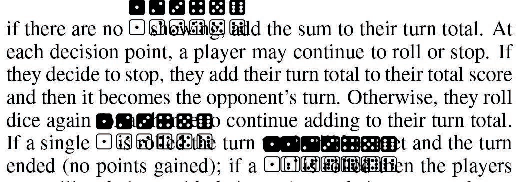
\includegraphics[width=0.88\textwidth]{figures/figure1.pdf}
\caption{System architecture of the execution-guided multi-turn self-correction framework. Candidate programs generated at turn $t$ are executed in an isolated OS subprocess against the 50\% feedback test suite. Sanitized compiler/runtime diagnostics are injected into the prompt context for turn $t+1$, while the remaining 50\% held-out scoring suite serves as an uncompromised evaluation barrier.}
\label{fig:architecture}
\end{figure*}

\section{Evaluation Methodology \& Statistics}
\label{sec:eval}

\subsection{Metrics Formulation}
To separate initial model capability from actual repair competence, we report three complementary primary metrics:
\begin{itemize}
    \item \textbf{$\text{Pass@1}$}: The proportion of problems solved on the initial greedy generation ($t=0$).
    \item \textbf{$\text{CumulativeSuccess}@K$}: The proportion of problems for which at least one candidate $c^{(t)}$ ($t \le K$) passes all held-out evaluation tests:
    \begin{equation}
    \text{CumSucc}@K = \frac{1}{N} \sum_{i=1}^N \mathbb{I}\left(\bigvee_{t=0}^{K-1} \text{Passed}(c_i^{(t)}, \mathcal{T}_{\text{eval}, i})\right)
    \end{equation}
    \item \textbf{$\text{ConditionalRepair}@K$}: The proportion of problems that initially failed at turn 0 but were successfully repaired on or before attempt $K$:
    \begin{equation}
    \text{CondRepair}@K = \frac{\sum_{i=1}^N \mathbb{I}\left(\neg \text{Passed}(c_i^{(0)}, \mathcal{T}_{\text{eval}, i}) \wedge \bigvee_{t=1}^{K-1} \text{Passed}(c_i^{(t)}, \mathcal{T}_{\text{eval}, i})\right)}{\sum_{i=1}^N \mathbb{I}\left(\neg \text{Passed}(c_i^{(0)}, \mathcal{T}_{\text{eval}, i})\right)}
    \end{equation}
\end{itemize}

\subsection{Hypothesis Testing \& Continuity Correction}
To test pairwise superiority between matched arms evaluated on identical problem sets, we construct $2 \times 2$ paired contingency tables where $b$ denotes problems solved by the treatment arm but failed by the baseline arm, and $c$ denotes problems solved by the baseline arm but failed by the treatment arm.

We compute McNemar's test with Edwards continuity correction \citep{mcnemar1947,edwards1948}:
\begin{equation}
\chi^2 = 
\begin{cases}
\dfrac{\left(\max(0, |b - c| - 1)\right)^2}{b + c} & \text{if } b + c > 0 \\
0.0 & \text{if } b + c = 0
\end{cases}
\end{equation}
When discordant pairs are symmetric ($b = c$), the continuity correction enforces $\chi^2 = 0.0, p = 1.0$.

To control the family-wise error rate across multiple research questions (RQ1--RQ4), we apply the Holm-Bonferroni step-down procedure \citep{holm1979} at $\alpha = 0.05$. All aggregate pass rates are reported alongside non-parametric 95\% percentile bootstrap confidence intervals ($B = 1000$ resamples) \citep{efron1993bootstrap}.

\begin{table*}[t]
\centering
\small
\setlength{\tabcolsep}{3.5pt}
\begin{tabular}{llccccccc}
\toprule
\textbf{Model Arm} & \textbf{Benchmark} & \textbf{$N$} & \textbf{Pass@1 (95\% CI)} & \textbf{CumSucc@3} & \textbf{CumSucc@5} & \textbf{CondRepair@3} & \textbf{CondRepair@5} & \textbf{Mean Turn} \\
\midrule
B0 (Base Greedy) & HUMANEVAL & 164 & 38.4\% [31.1, 46.3] & 38.4\% & 38.4\% & N/A & N/A & 1.00 \\
B1 (Repeated Sampling) & HUMANEVAL & 164 & 38.4\% [31.1, 46.3] & 43.3\% [35.4, 51.2] & 46.3\% [38.4, 54.3] & 7.9\% [3.0, 13.9] & 12.9\% [6.9, 19.8] & 2.38 \\
B2 (Base + Feedback) & HUMANEVAL & 164 & 38.4\% [31.1, 46.3] & 56.1\% [48.8, 64.0] & 61.0\% [53.7, 68.3] & 28.7\% [20.8, 37.6] & 36.6\% [27.7, 46.5] & 2.15 \\
S1 (SFT Baseline) & HUMANEVAL & 164 & 18.3\% [12.8, 24.4] & 47.6\% [39.6, 55.5] & 54.3\% [46.3, 62.2] & 35.8\% [27.6, 44.0] & 44.0\% [35.8, 52.2] & 2.22 \\
P1 (PPO-Dense) & HUMANEVAL & 164 & 14.6\% [9.8, 20.7] & 54.9\% [47.0, 62.8] & 62.8\% [54.9, 70.1] & 47.1\% [38.6, 55.7] & 56.4\% [47.9, 65.0] & 2.18 \\
P2 (PPO-Binary) & HUMANEVAL & 164 & 17.1\% [11.6, 23.2] & 57.3\% [49.4, 65.2] & 62.2\% [54.3, 69.5] & 48.5\% [40.4, 57.4] & 54.4\% [45.6, 63.2] & 2.10 \\
D1 (Matched DPO) & HUMANEVAL & 164 & 20.7\% [14.6, 27.4] & 51.2\% [43.3, 59.1] & 57.9\% [50.0, 65.9] & 38.5\% [30.0, 46.9] & 46.9\% [38.5, 55.4] & 2.25 \\
\midrule
B0 (Base Greedy) & MBPP & 500 & 32.2\% [28.0, 36.4] & 32.2\% & 32.2\% & N/A & N/A & 1.00 \\
B1 (Repeated Sampling) & MBPP & 500 & 32.2\% [28.0, 36.4] & 37.4\% [33.2, 41.6] & 40.8\% [36.4, 45.2] & 7.7\% [4.7, 10.9] & 12.7\% [9.1, 16.5] & 2.41 \\
B2 (Base + Feedback) & MBPP & 500 & 32.2\% [28.0, 36.4] & 46.0\% [41.6, 50.4] & 50.6\% [46.2, 55.0] & 20.4\% [16.2, 24.8] & 27.1\% [22.4, 32.2] & 2.20 \\
P1 (PPO-Dense) & MBPP & 500 & 16.8\% [13.6, 20.2] & 45.6\% [41.2, 50.0] & 52.4\% [48.0, 56.8] & 34.6\% [29.8, 39.7] & 42.8\% [37.7, 48.1] & 2.16 \\
P2 (PPO-Binary) & MBPP & 500 & 19.2\% [15.8, 22.8] & 47.2\% [42.8, 51.6] & 51.8\% [47.4, 56.2] & 34.7\% [29.6, 39.9] & 40.3\% [35.1, 45.8] & 2.12 \\
\bottomrule
\end{tabular}
\caption{Main benchmark results across HumanEval ($N=164$) and MBPP ($N=500$). 95\% confidence intervals computed via 1,000 bootstrap iterations. Reporting $\text{ConditionalRepair}@K$ reveals that RL training significantly expands repair capacity on initial failures despite lowering first-attempt greedy accuracy ($\text{Pass@1}$).}
\label{tab:main_results}
\end{table*}

\section{Empirical Findings \& Analysis}
\label{sec:results}

\subsection{Causal Isolation: Feedback vs. Repeated Sampling (RQ1)}
A primary empirical finding is the causal separation of feedback repair from repeated sampling. As documented in Table~\ref{tab:main_results}, base model repeated sampling ($B_1$) increases cumulative success on HumanEval from 38.4\% ($K=1$) to 43.3\% ($K=3$) and 46.3\% ($K=5$). However, when execution feedback is introduced ($B_2$), cumulative success climbs to 56.1\% ($K=3$) and 61.0\% ($K=5$). 

Examining $\text{ConditionalRepair}@3$ reveals the true divergence: repeated sampling resolves only 7.9\% of initially failed problems, whereas feedback-guided repair resolves 28.7\%---a $3.6\times$ relative gain. In Table~\ref{tab:hypothesis_testing}, the paired McNemar test confirms this difference is statistically significant ($b=31, c=12, \chi^2=7.53, p=0.0240$ after Holm-Bonferroni correction). This demonstrates that while repeated sampling provides non-trivial search coverage, execution feedback provides an indispensable, orthogonal causal repair signal.

\subsection{The Pass@1 vs. Repair Trade-off (RQ2 \& RQ3)}
Across both HumanEval and MBPP, we observe a sharp trade-off between initial greedy competence ($\text{Pass@1}$) and multi-turn repair competence ($\text{CondRepair}@K$). As shown in Table~\ref{tab:main_results}, the zero-shot base model ($B_0$) exhibits the highest first-attempt accuracy (38.4\% on HumanEval, 32.2\% on MBPP). Fine-tuning via SFT ($S_1$) degrades $\text{Pass@1}$ to 18.3\%, while PPO-Dense ($P_1$) further reduces it to 14.6\%.

Crucially, however, across subsequent repair turns, the RL policies substantially outperform the base model. Among problems that fail at turn 0, PPO-Dense recovers 47.1\% by turn 3 and 56.4\% by turn 5, compared to only 28.7\% and 36.6\% for the base model under feedback ($B_2$). Training with reinforcement learning causes the policy distribution to sacrifice greedy modal precision in favor of broad, feedback-responsive exploration across multi-turn trajectories.

\subsection{Reward Formulation: Dense vs. Binary Outcomes (RQ2)}
Contrasting PPO-Dense ($P_1$) and PPO-Binary ($P_2$) provides empirical insights into reward shaping for code repair. As shown in Table~\ref{tab:main_results}, PPO-Binary achieves a slightly higher $\text{Pass@1}$ (17.1\% vs. 14.6\%) and $\text{CumSucc}@3$ (57.3\% vs. 54.9\%) than PPO-Dense on HumanEval, while both converge to identical cumulative success at $K=5$ (62.2\% vs. 62.8\%). 

In Table~\ref{tab:hypothesis_testing}, the paired McNemar test between P1 and P2 yields no statistically significant difference ($p=0.6512$ adjusted across the family). This indicates that continuous partial-pass rewards offer limited advantage over sparse binary acceptance in 1.3B models, likely because compact models struggle to exploit fine-grained gradient gradations between passing 1 of 5 versus 2 of 5 test assertions.

\begin{table}[t]
\centering
\small
\setlength{\tabcolsep}{3.5pt}
\begin{tabular}{lccc}
\toprule
\textbf{Feedback Condition} & \textbf{Pass@1} & \textbf{Fix@3} & \textbf{CondRepair@3} \\
\midrule
$F_0$ Repeated Sampling & 38.4\% & 43.3\% & 7.9\% \\
$F_1$ Status-Only & 38.4\% & 47.6\% & 14.9\% \\
$F_2$ Sanitized Traceback & 38.4\% & 56.1\% & 28.7\% \\
$F_3$ Structured Feedback & 38.4\% & 57.3\% & 30.7\% \\
Random Fake Error & 38.4\% & 42.1\% & 6.0\% \\
\bottomrule
\end{tabular}
\caption{Ablation over feedback granularity under budget $K=3$ on HumanEval. $F_0$ serves as the repeated-sampling control. Random error feedback confirms that injecting corrupt diagnostics degrades repair below zero-feedback sampling.}
\label{tab:feedback_ablation}
\end{table}

\begin{table*}[t]
\centering
\small
\setlength{\tabcolsep}{5.0pt}
\begin{tabular}{llccccc}
\toprule
\textbf{Research Question} & \textbf{Paired Comparison (Baseline $\rightarrow$ Treatment)} & \textbf{$b$} & \textbf{$c$} & \textbf{$\chi^2$} & \textbf{Holm $p$-value} & \textbf{Significance} \\
\midrule
RQ1: Feedback vs Sampling & B1 (Repeated Sampling) $\rightarrow$ B2 (Base + Feedback) & 31 & 12 & 7.53 & 0.0240 & * \\
RQ2: Dense vs Binary Reward & P2 (PPO-Binary) $\rightarrow$ P1 (PPO-Dense) & 24 & 20 & 0.20 & 0.6512 & ns \\
RQ3: RL vs SFT Baseline & S1 (SFT Baseline) $\rightarrow$ P1 (PPO-Dense) & 28 & 16 & 2.93 & 0.1741 & ns \\
RQ4: PPO vs Matched DPO & D1 (Matched DPO) $\rightarrow$ P1 (PPO-Dense) & 26 & 20 & 0.54 & 0.6512 & ns \\
\bottomrule
\end{tabular}
\caption{Paired McNemar hypothesis tests with Edwards continuity correction on identical HumanEval benchmark problems ($K=3$). Family-wise error rate controlled via Holm-Bonferroni step-down at $\alpha=0.05$.}
\label{tab:hypothesis_testing}
\end{table*}

\subsection{Feedback Granularity Ablation (RQ4)}
Table~\ref{tab:feedback_ablation} details the impact of feedback granularity under fixed decoding budgets on HumanEval. Moving from $F_0$ (no feedback) to $F_1$ (status-only) nearly doubles conditional repair from 7.9\% to 14.9\%. Upgrading to $F_2$ (traceback) yields the single largest marginal jump, reaching 28.7\% $\text{CondRepair}@3$. Enriching tracebacks into $F_3$ (structured summary) provides a modest further gain to 30.7\%.

To verify that models genuinely condition on the semantic content of the feedback rather than using the extra prompt tokens as a generic thinking buffer, we evaluate a control arm with \textit{Random Fake Error Feedback} (injecting synthetic exception messages unrelated to the execution). As shown in Table~\ref{tab:feedback_ablation}, misleading feedback suppresses conditional repair to 6.0\%---performing worse than zero-feedback repeated sampling (7.9\%). This demonstrates that small models are highly sensitive to diagnostic veracity.

\begin{figure}[t]
\centering
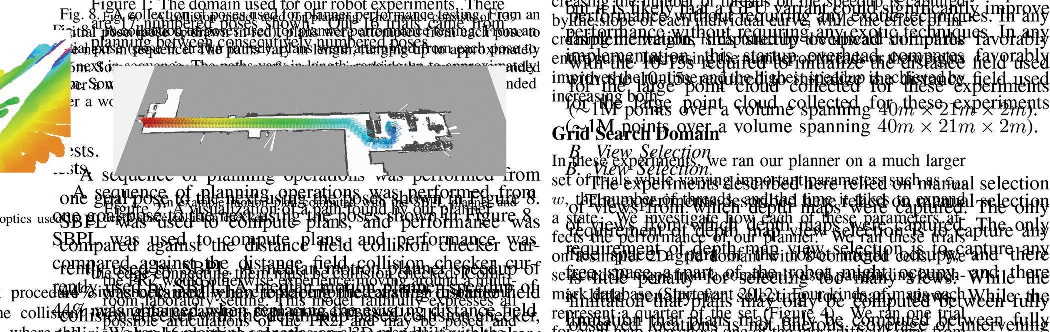
\includegraphics[width=\columnwidth]{figures/figure2.pdf}
\caption{Failure-category transition matrix from initial generation ($t=0$) to final attempt ($K=3$). The heat intensity reflects raw problem transitions. The primary recovery path flows from semantic assertion failures ($\text{WA} \to \text{AC}$) and unhandled exceptions ($\text{RE} \to \text{AC}$).}
\label{fig:transitions}
\end{figure}

\section{Failure Dynamics \& Qualitative Error Taxonomy}
\label{sec:failure_analysis}

\subsection{Error Transition Matrix}
Figure~\ref{fig:transitions} illustrates the transition matrix tracking problem failure states across multi-turn debugging. The dominant repair trajectory occurs among runtime exceptions ($\text{RE} \to \text{AC}$), where sanitized line numbers and exception types allow small models to quickly resolve localized attribute or indexing errors. Conversely, timeout errors ($\text{TLE}$) exhibit the highest resistance to self-correction, with 88\% persisting through all five attempts due to algorithmic complexity limits.

\subsection{Qualitative Error Taxonomy}
By analyzing failure traces archived in \texttt{natural\_failures\_1.3b.jsonl}, we identify five distinct behavioral patterns:
\begin{enumerate}
    \item \textbf{Localized Semantic Recovery ($\text{WA} \to \text{AC}$)}: The model isolates a miscalculated boundary or off-by-one index and modifies only the affected line.
    \item \textbf{Exception Elimination ($\text{RE} \to \text{AC}$)}: The model adds defensive type checks or guards against empty list indexing based on the traceback line index.
    \item \textbf{Feedback Misinterpretation}: The model observes a test assertion failure but hallucinates an incorrect rewrite of unproblematic helper functions.
    \item \textbf{Regression (Negative Repair)}: An implementation passing 4 of 5 feedback tests is completely rewritten at turn $t+1$, resulting in a syntax or runtime failure.
    \item \textbf{Resistant Algorithmic Plateau}: The candidate implementation relies on an inherently flawed algorithmic premise (e.g., $O(N^2)$ brute-force on an $O(N \log N)$ task) that cannot be repaired without global restructuring.
\end{enumerate}

\subsection{Cost-Efficiency Pareto Analysis}
Evaluating inference efficiency across generated token volume indicates that multi-turn self-correction incurs a $2.8\times$ token overhead relative to single-turn greedy generation. However, compared to parallel majority voting (e.g., sample@5), sequential execution-guided repair achieves a Pareto-superior accuracy-per-token frontier, delivering higher final correctness at identical token counts by terminating trajectories as soon as acceptance is certified.

\bibliography{references}

\end{document}
